\documentclass[main.tex]{subfiles}

\begin{document}

\chapter{Problem 1.2 - Constrained Optimization}

\section{Problem Description}

This task is split on two parts a) and b). Goal of part a) is to find global minimum of objective function constrained by closed set using analytical method, and goal of part b) is to determine minimum and corresponding function value of constrained objective function using Lagrange Multipler Method.


\newpage
\section{Part a) - Analytical Method}

\subsection{Problem Introduction}
As described above problem is to find a global minimum of objective function:
\begin{equation}
    f(x_1,x_2)=4*x_1^2-x_1*x_2+4*x_2^2-6*x_2
\end{equation}
subject to closed set $S$ defined as triangle by corner points located at (0,0), (0,1) and (1,1). Describing problem graphically, one may present it as on figure \ref{fig:analyticalProblem}.

\begin{figure}[h]
\label{fig:solution}
\centering
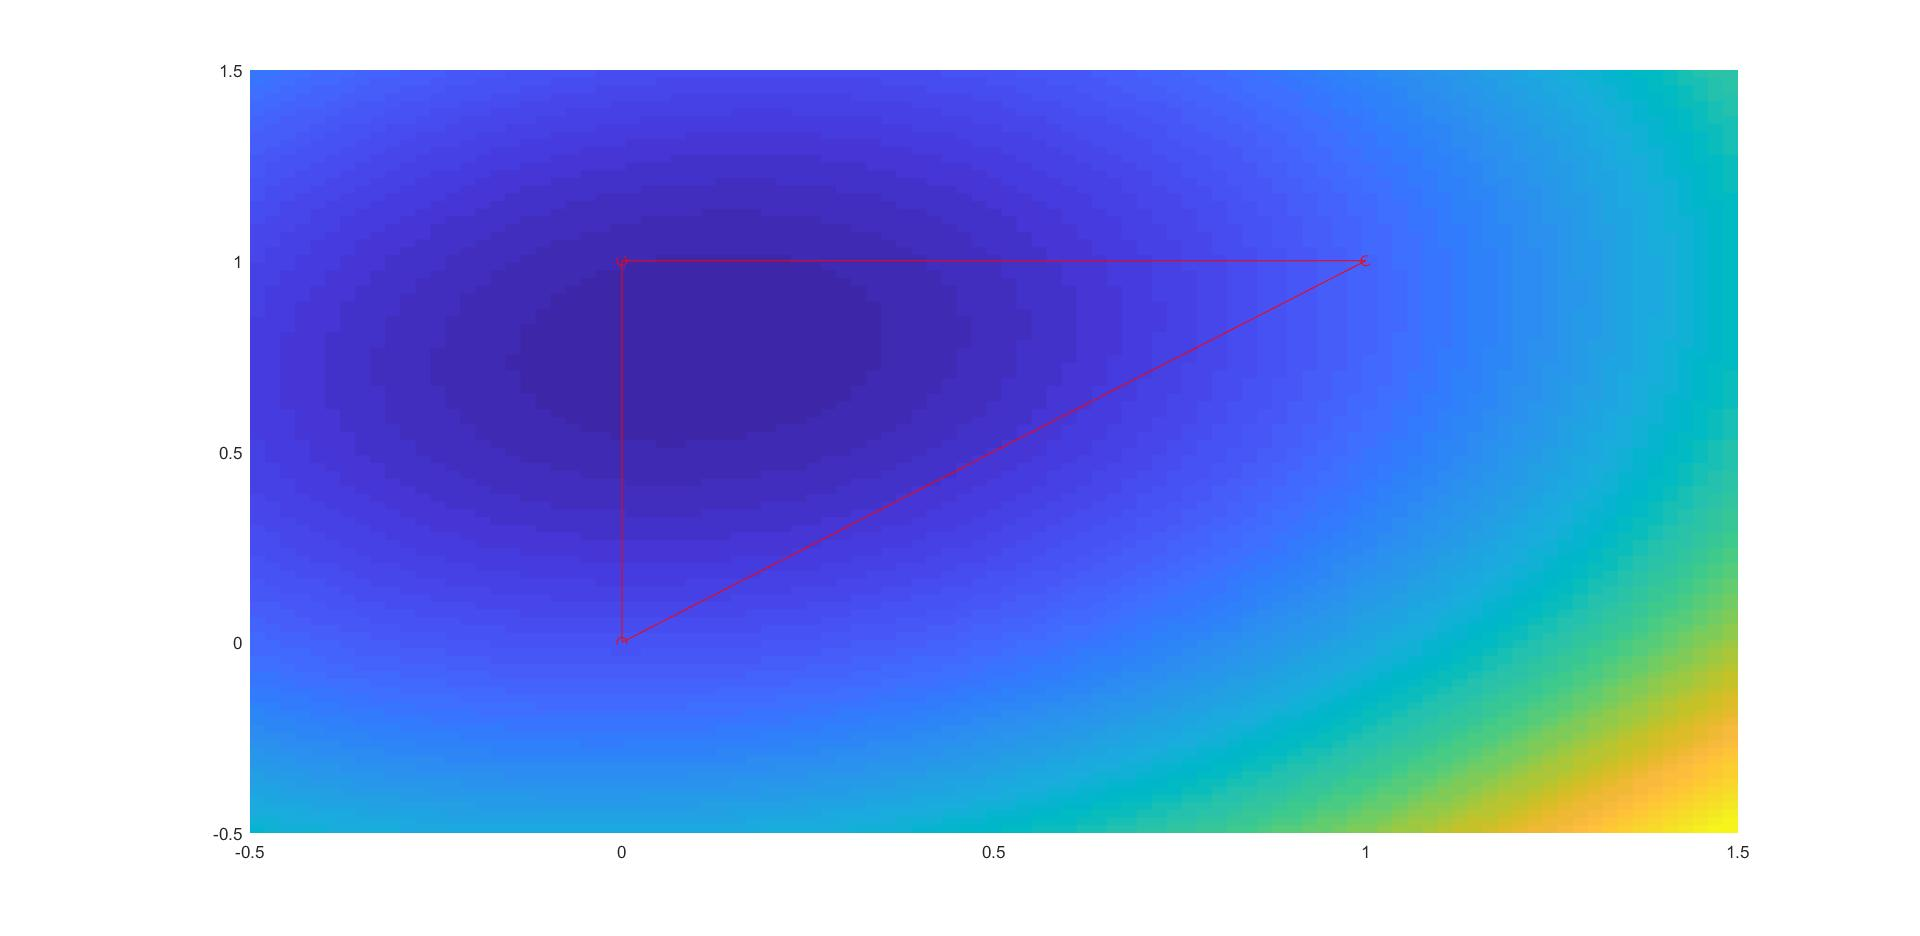
\includegraphics[width=\textwidth]{AnalyticalMethod/ObjectiveFunctionAndClosedSet.jpg}
\label{fig:analyticalProblem}
\caption{Objective Function $f(x_1,x_2)=4*x_1^2-x_1*x_2+4*x_2^2-6*x_2$ and closed set $S$}
\end{figure}

\newpage
\subsection{Solution Methodology}
Steps to solve this problem are as follows:
\begin{enumerate}
    \item First find stationary points $\vec{x}_{(SP)}^{*}$ of objective function on interior of closed set $S$. This is done by gradient of objective function compared to zero.
    \item Then find stationary points $\vec{x}_{(SP)}^{*}$ on boundary $\partial{S}$ of closed set $S$. For this use objective function to obtain functions of lines between each pair of corner points of triangle describing closed set $S$. Then get gradients for set of this line functions and solve for gradients equal to zero.
    \item Next find stationary points $\vec{x}_{(SP)}^{*}$ on corner points of triangle of closed set $S$.
    \item Lastly for each pair of stationary points $\vec{x}_{(SP)}^{*}$ select point which will give minimum objective function value. This is global minimum and solution to problem.
\end{enumerate}

\newpage
\subsection{Stationary Points $\vec{x}_{(SP)}^{*}$ of $f(\vec{x})$ on closed set $S$}

To find stationary point of function, by definition we compare gradient of this function to zero

\begin{equation}
\nabla{f(x_1,x_2)} = \left(
\frac{\partial{f(x_1,x_2)}}{\partial{x_1}}, \frac{\partial{f(x_1,x_2)}}{\partial{x_2}}
\right) = 0
\end{equation}

\begin{equation}\left \{
\begin{tabular}{l}
$\frac{\partial{f(x_1,x_2)}}{\partial{x_1}} = 8*x_1 - x_2 + 0 - 0 = 0$\\
$\frac{\partial{f(x_1,x_2)}}{\partial{x_2}} = 0 - x_1 + 8*x_2 - 6 = 0$\\
\end{tabular}\right
\end{equation}

then solving this simple equation system

\begin{equation}\left \{
\begin{tabular}{lclcl}
$8*x_1 - x_2 + 0 - 0 = 0$&$\Leftrightarrow$&$x_2 = 8*x_1$&$\Leftrightarrow$&$x_2=48/63$ \\
$x_1 + 8*(8*x_1) - 6 = 0$&$\Leftrightarrow$&$x_1 = 6/63$ & &\\
\end{tabular}\right
\end{equation}

one finds stationary point $\vec{x}_{(SP1)}^{*}=(6/63,48/63)$ in interior of closed set domain over objective function.

\newpage
\subsection{Stationary Points $\vec{x}_{(SP)}^{*}$ of $f(\vec{x})$ on closed set boundary $\partial{S}$}

To obtain stationary points on boundary of closed set it is sufficient to define 3 lines between 3 pairs of corner points (0,0), (0,1) and (1,1) creating triangle edges what is geometrical representation of closed set $S$ boundary.

\subsubsection{Line from (0,0) to (0,1) }

Line connecting points (0,0) and (0,1) is deduced as follows:

\begin{equation}\left \{
\begin{tabular}{l}
$x_1=0;$\\
$0 < x_2 < 1;$\\
\end{tabular}\right
\end{equation}

Binomial objective function $f(x_1,x_2)$ for this values take form of monomial function $f(x_1=0, 0<x_2<1) = f(0<x_2<1)$:

\begin{equation}
    f(x_2) = 4*0^2 - 0*x_2 + 4*x_2^2 - 6*x_2 \quad \forall x_2 \in [0,1]
\end{equation}

for which gradient is reduced to first derivative and compared to zero

\begin{equation}
    f'(x_2) = 8*x_2 - 6 = 0
\end{equation}

and solved, gives stationary point $\vec{x}_{(SP2)}^{*} = (0, 6/8)$.

\subsubsection{Line from (0,1) to (1,1) }

Line between pair of corners (0,1) and (1,1) is similarly:

\begin{equation}\left \{
\begin{tabular}{l}
$0 < x_1< 1;$\\
$x_2 = 1;$\\
\end{tabular}\right
\end{equation}

Binomial objective function $f(x_1,x_2)$ for this values take form of monomial function $f(0<x_1<1, x_2 = 1) = f(0<x_1<1)$:

\begin{equation}
\begin{split}
f(x_1) & = 4*x_1^2 - x_1*1 + 4*1^2 - 6*1 \\
       & = 4*x_1^2 - x_1 + -2 \\
\end{split}
\end{equation}

where $f(x_1) \quad \forall x_1 \in [0,1]$ and for which gradient is reduced to first derivative, then compared to zero

\begin{equation}
    f'(x_2) = 8*x_1 - 1 = 0
\end{equation}

Solving this equality, gives stationary point $\vec{x}_{(SP3)}^{*} = (1/8, 1)$.


\subsubsection{Line from (0,0) to (1,1) }

Lastly line from point (0,0) to point (1,1) is defined:

\begin{equation}\left \{
\begin{tabular}{l}
$0 < x_1< 1;$\\
$0 < x_2 < 1;$\\
\end{tabular}\right
\end{equation}

or simplifying

\begin{equation}\left \{
\begin{tabular}{l}
$x_1=x_2;$\\
$x_2;$\\
\end{tabular}\right
\end{equation}

Binomial objective function $f(x_1,x_2)$ for this values take form of monomial function $f(x_2)$:

\begin{equation}
\begin{split}
f(x_2) & = 4*x_2^2 - x_2*x_2 + 4*x_2^2 - 6*x_2 \\
       & = 7*x_2^2 - 6*x_2 \\
\end{split}
\end{equation}

where $f(x_2) \quad \forall x_2 \in [0,1]$ and for which gradient is reduced to first derivative, then compared to zero

\begin{equation}
    f'(x_2) = 14*x_2 - 6 = 0
\end{equation}

Solving this equality, gives stationary point $\vec{x}_{(SP4)}^{*} = (3/7, 3/7)$.

\newpage

\subsection{Stationary Points $\vec{x}_{(SP)}^{*}$ of $f(\vec{x})$ on closed set $S$ corner points (0,0), (0,1) and (1,1)}

\subsubsection{Stationary Point on corner (0,0)}

\begin{equation}
f(x_1=0,x_2=0) = 0
\end{equation}

so gradient $f'(x_1=0,x_2=0) = 0$ and $\vec{x}_{(SP5)}^{*} = (0,0)$


\subsubsection{Stationary Point on corner (0,1)}

\begin{equation}
f(x_1=0,x_2=1) = 4*0 - 0*1 + 4*1 - 6*1 = - 2
\end{equation}

so gradient $f'(x_1=0,x_2=1) = 0$ and $\vec{x}_{(SP6)}^{*} = (0,1)$


\subsubsection{Stationary Point on corner (1,1)}

\begin{equation}
f(x_1=1,x_2=1) = 4*1 - 1*1 + 4*1 - 6*1 = 1
\end{equation}

so gradient $f'(x_1=1,x_2=1) = 0$ and $\vec{x}_{(SP7)}^{*} = (1,1)$

\newpage
\subsection{Results}

Grouping acquired stationary points and corresponding to them function values to table \ref{tab:analyticalMethodResults}, it is easy to distinguish that global minima is at point (2/21,16/21) with value -2.285.

\begin{table}[h]
\centering
\begin{tabular}{l | c | c | c }
n & x_1 & x_2 & $f(\vec{x})$\\
\hline \hline
1&	2/21&16/21&-2.285\\
2&	0& 	 6/8&  -2.25\\
3&	1/8& 1&    -2.0625\\
4&	3/7& 3/7&  -1.285\\
5&	0&	 0&     0\\
6&	0&	 1&    -2\\
7&	1&	 1&     1\\
\end{tabular}

\caption{Stationary Points and corresponding objective function values obtained by Analytical Method}
\label{tab:analyticalMethodResults}
\end{table}

\begin{figure}[h]
\centering
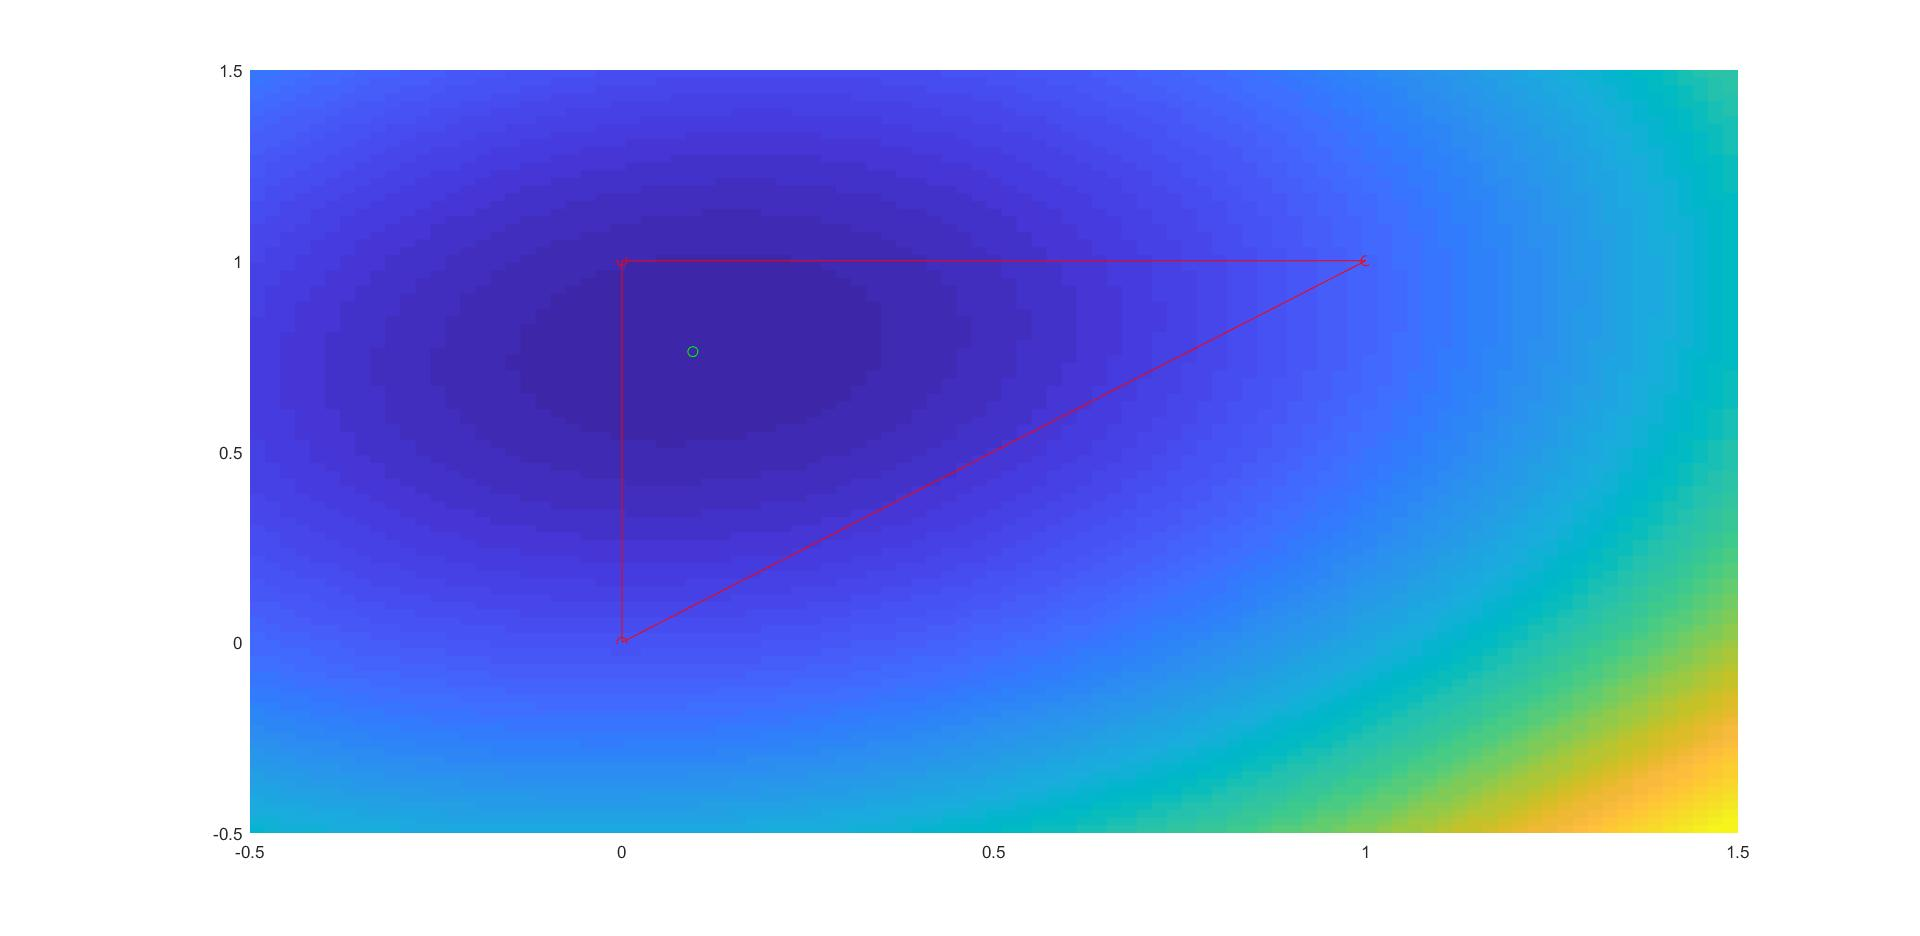
\includegraphics[width=\textwidth]{AnalyticalMethod/ObjectiveFunctionAndClosedSet_Minima.jpg}
\label{fig:solution}
\caption{Stationary Point (marked with circle) of global minima of objective function in closed set $S$)}
\end{figure}

\newpage

\subsection{Conclusions}

Analytical Method is based on properties of gradient of continuous differentable function. Its methodology is simple, depends on obtaining stationary points and value of this points in objective function. It may be seen that obtained global minima of function constrained by set $S$ is equal to unconstrained function flobal minimum. From this one may deduce, that it is sufficient to find global minima of function and if it is in valid domain of closed set, this minima would give solution to problem. If its not, one need to search for other stationary points, line in corners of boundary or on boundary.

\newpage
\section{Part b) - Lagrange Multipler Method}

\subsection{Problem Introduction}

In this task one has to use the Lagrange multiplier method (pp. 25-28 in the course book) to determine the minimum $(x_1^{*},x_2^{*})^T$ (as well as the corresponding function value) of the function $f(x_1,x_2) = 15 + 2*x_1 + 3*x_2$ subject to the equality constraint $h(x_1,x_2) = x^2_1 + x_1*x_2 + x_2^2 - 21 = 0$. Problem is represented graphically on figures \ref{fig:lagrangeFigsIntro}.

\begin{figure}[H]
\label{fig:lagrangeFigsIntro}
\centering
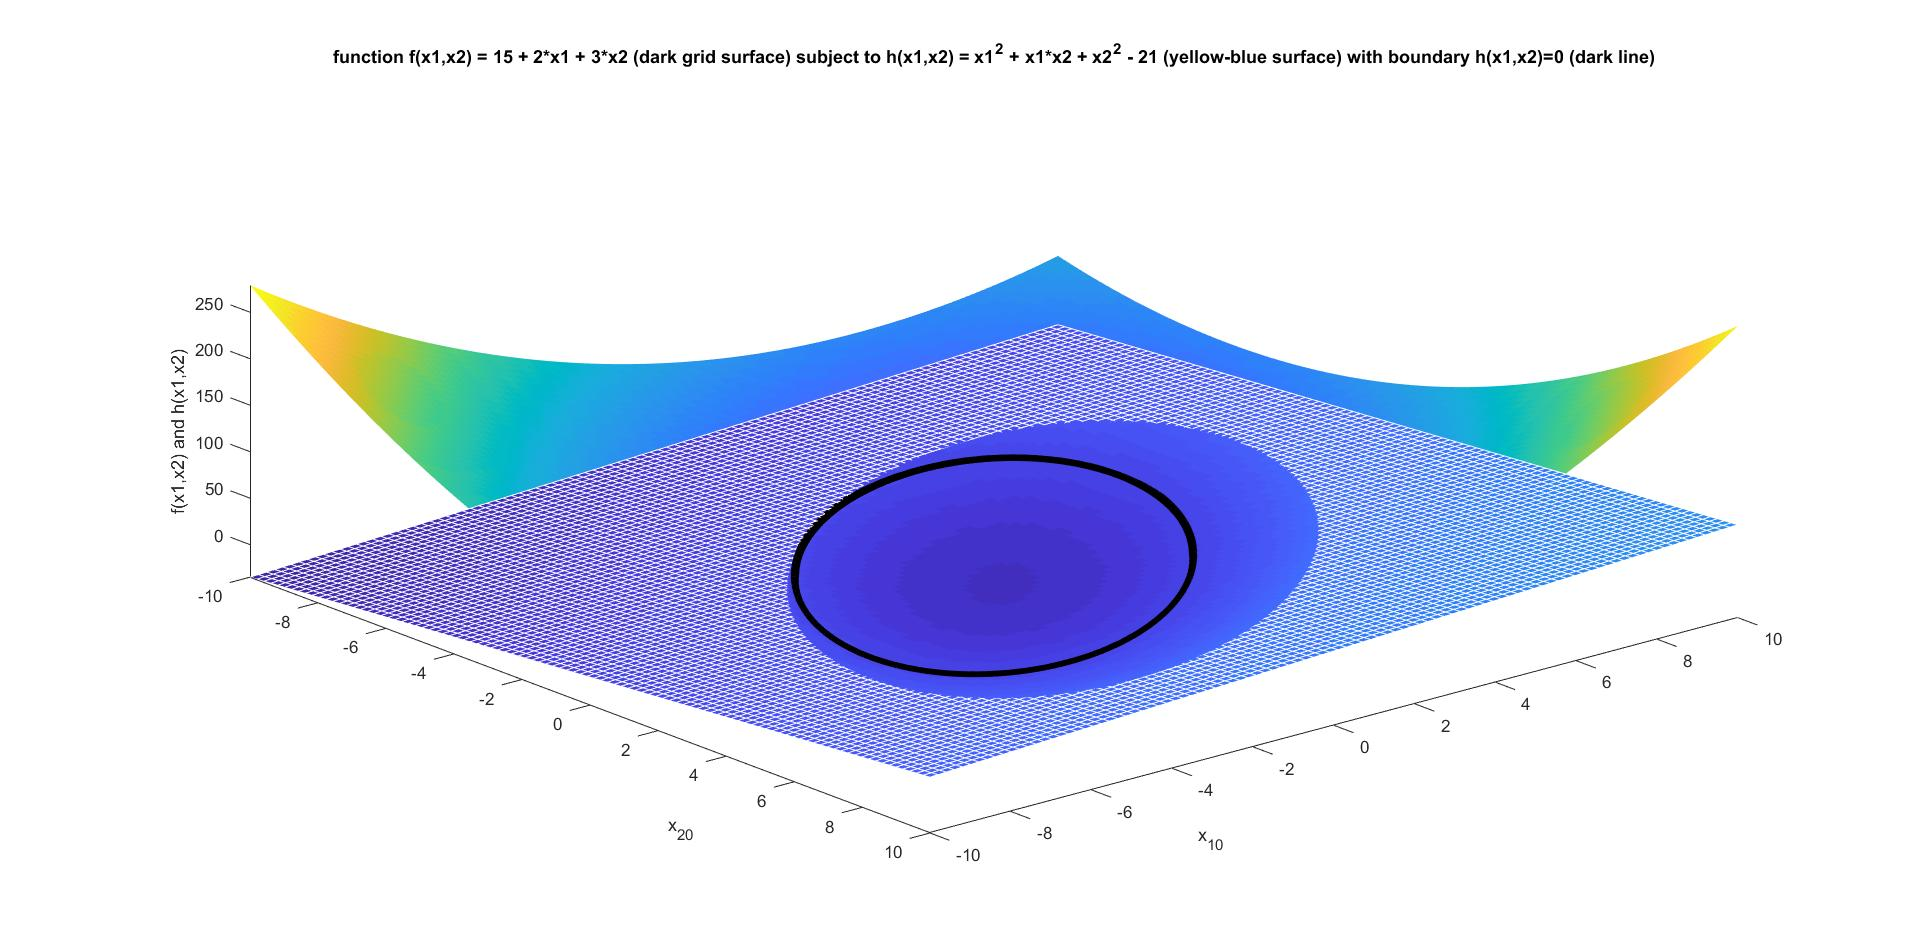
\includegraphics[width=\textwidth]{LagrangeMultiplerMethod/LagrangeMethod.jpg}
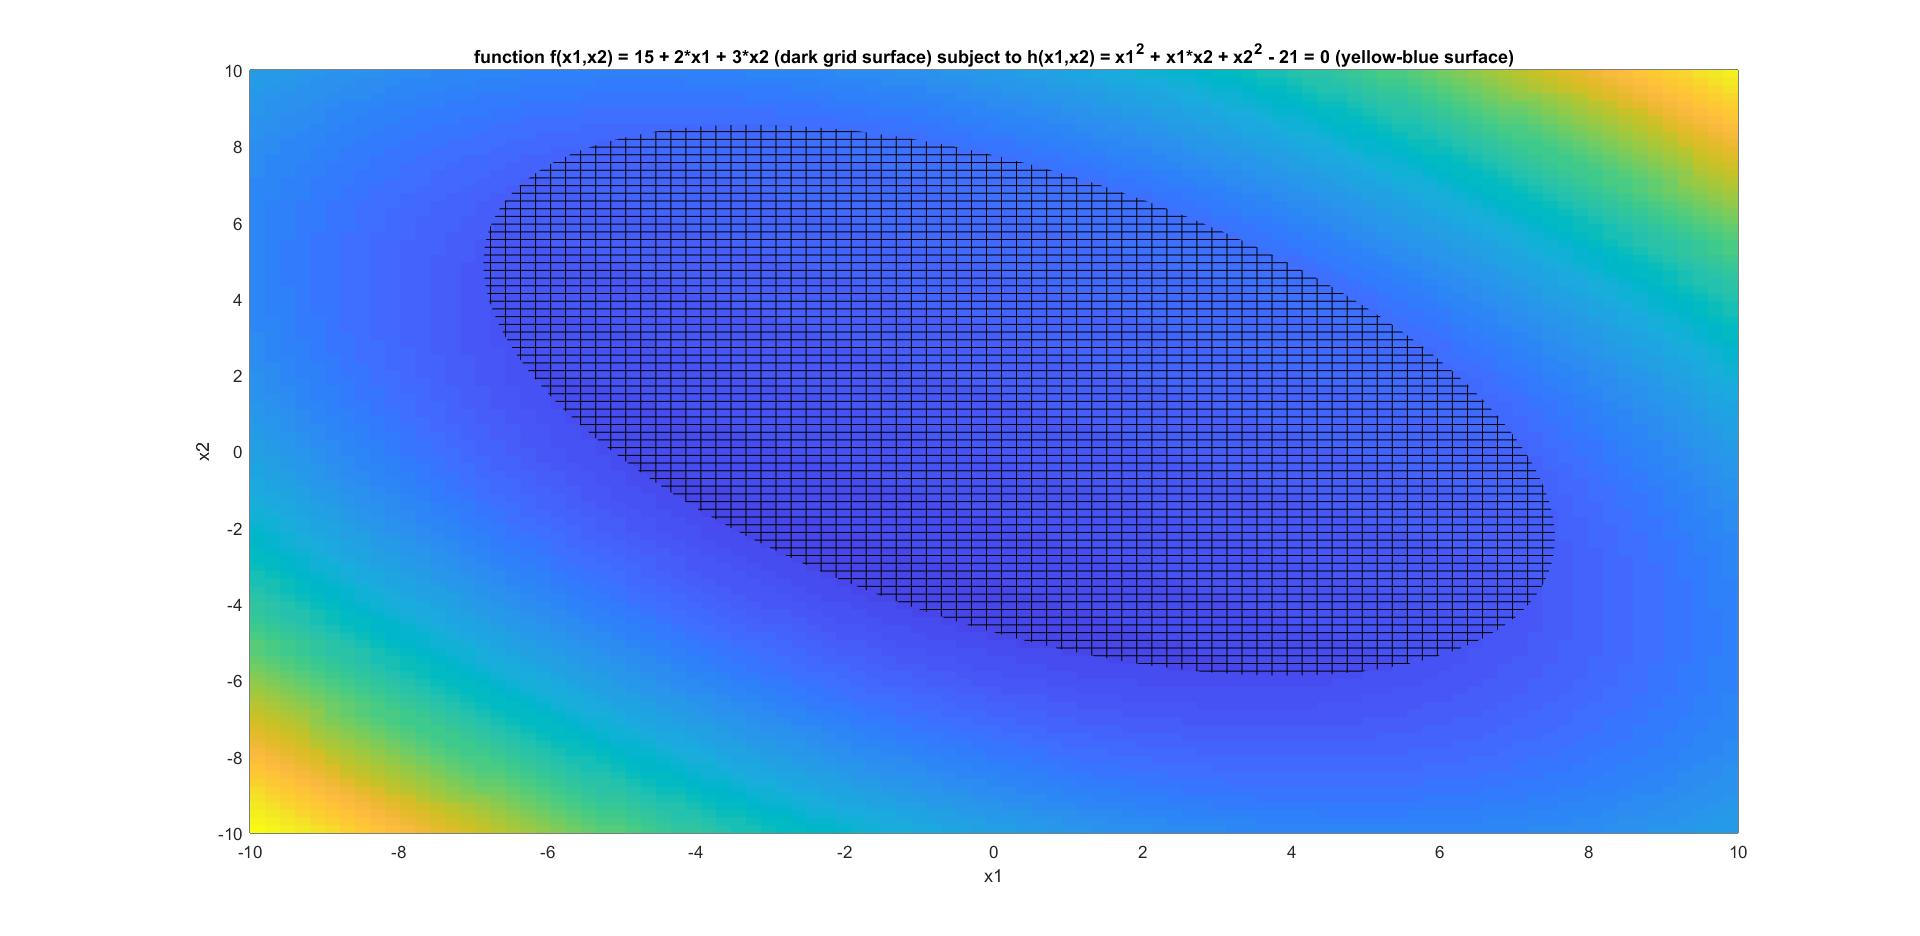
\includegraphics[width=\textwidth]{LagrangeMultiplerMethod/LagrangeMethod_view(0,90).jpg}
\caption{Objective function $f(x_1,x_2) = 15 + 2*x_1 + 3*x_2$ with equality constraint $h(x_1,x_2) = x^2_1 + x_1*x_2 + x_2^2 - 21 = 0$ (bottom picture in vertical view).}
\end{figure}

This task is solved as follows. 
\begin{enumerate}
    \item First form problem as Lagrange Multipler unconstrained function, transforming objective function and constraints.
    \item Next compare gradient of unconstrained function obtained in previous step.
    \item Thirdly solve for variables $x_1, x_2$ and if these variables happens to be in denominator go to step (4.) otherwise go to step (5.)
    \item Compare denominator to zero and solve for variables. Check if in this point function have optima.
    \item Select point with maximum/minimum function value as our maximum/minimum in question of problem. 
\end{enumerate}

\subsection{Lagrange Multipler unconstrained function}

Rewriting objective function and its constraint to Lagrange form

\begin{equation}
    L(\vec{x},\lambda) = f(\vec{x}) + \lambda*h(\vec{x})
\end{equation}

one obtains:

\begin{equation}
\begin{split}
 L(x_1,x_2,\lambda)  &  = f(x_1,x2) + \lambda*h(x_1,x_2) \\
       & = 15 + 2x_1 + 3x_2 + \lambda*(x^2_1 + x_1x_2 + x_2^2 - 21) \\
\end{split}
\end{equation}

what is graphically as on figures (for different values of $\lambda$)

\begin{figure}[H]
\label{fig:lagrangeEquationFigs1View90}
\centering
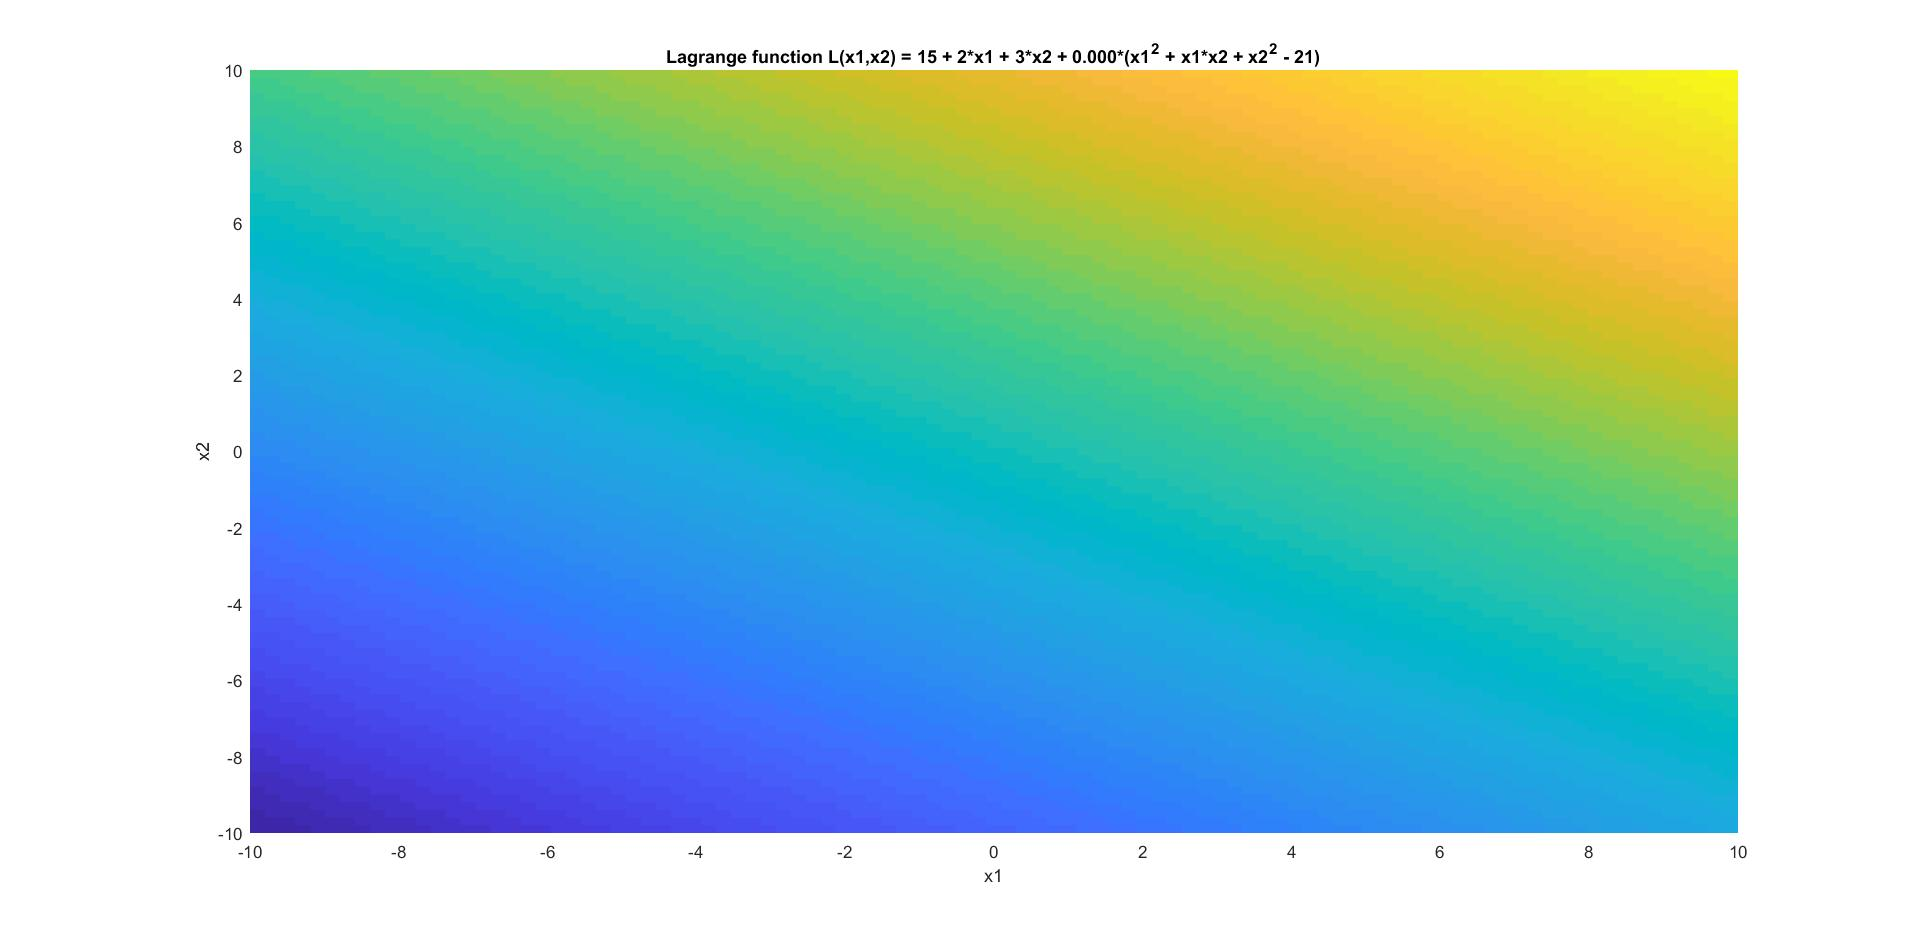
\includegraphics[width=\textwidth]{LagrangeMultiplerMethod/LagrangeMethod_equation_lambda=0.jpg}
\includegraphics[width=\textwidth]{LagrangeMultiplerMethod/{LagrangeMethod_equation_lambda=0.1}.jpg}
\includegraphics[width=\textwidth]{LagrangeMultiplerMethod/{LagrangeMethod_equation_lambda=0.333}.jpg}
\caption{Lagrange multiplier function $L(x_1,x_2,\lambda) = f(x_1,x2) + \lambda*h(x_1,x_2)$ for sequence of $\lambda$ values $[0,1/10,1/3]$ with vertical view on plane $(x_1,x_2)$.}
\end{figure}

\begin{figure}[H]
\label{fig:lagrangeEquationFigs2View90}
\centering
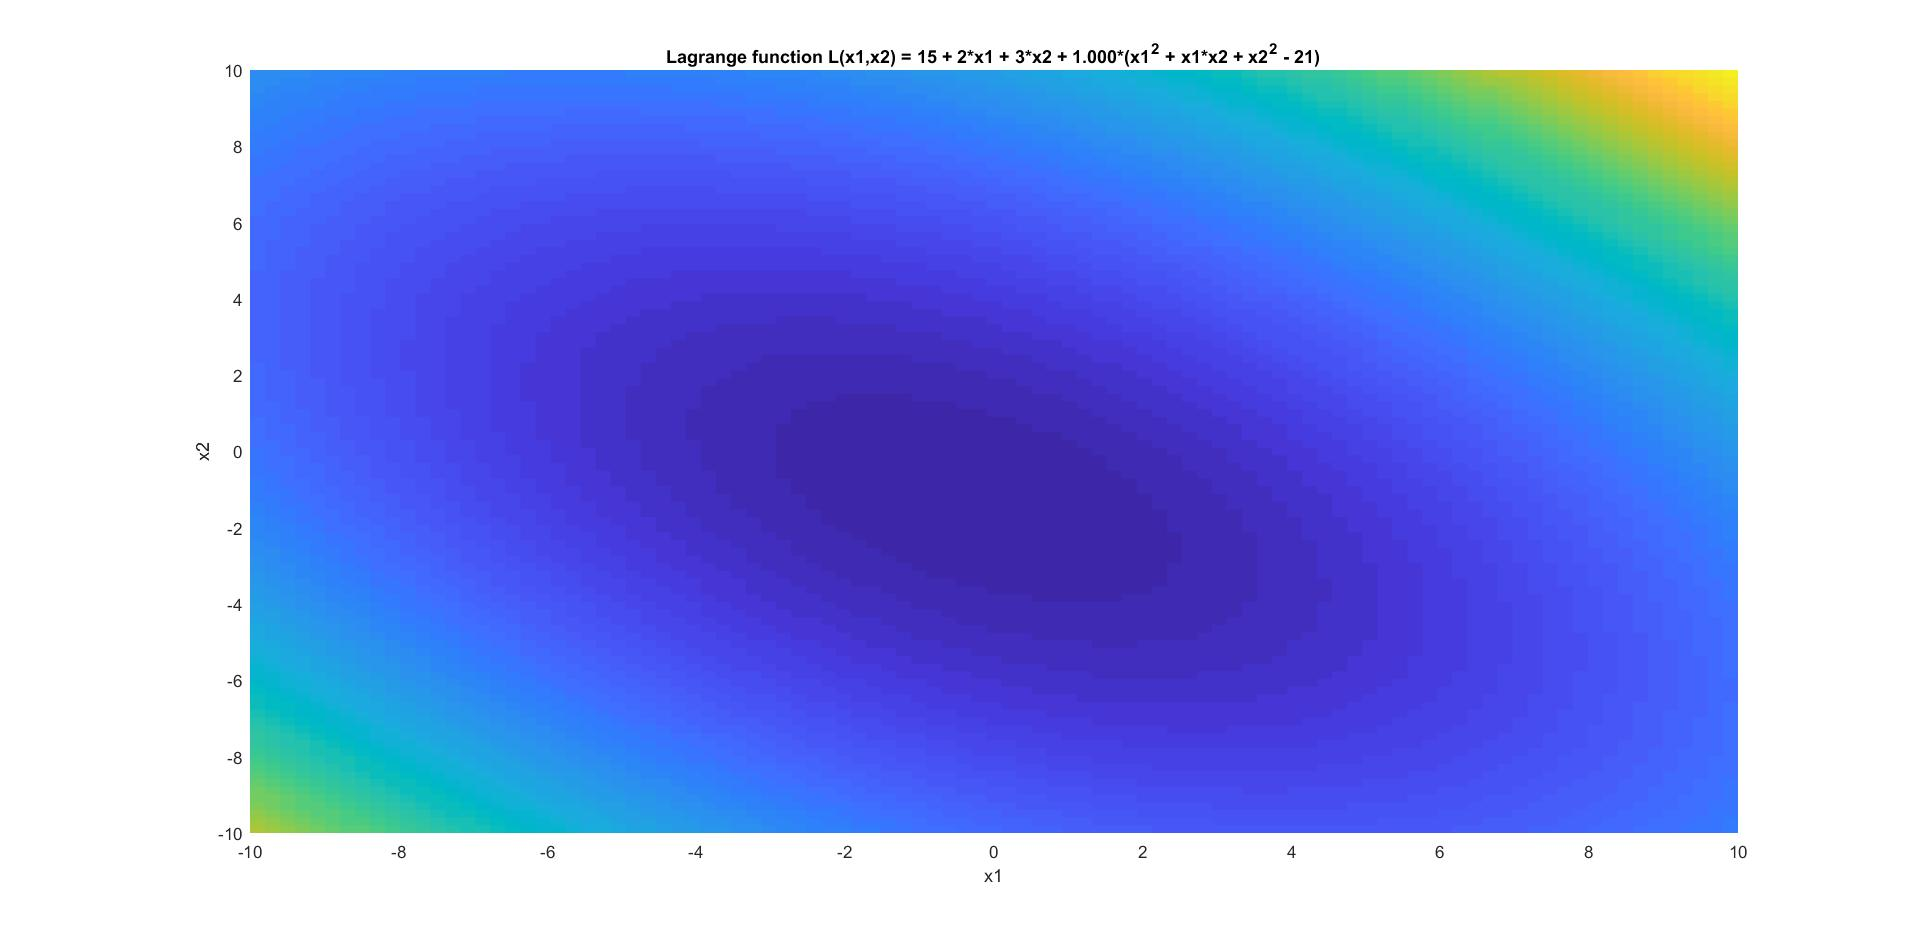
\includegraphics[width=\textwidth]{LagrangeMultiplerMethod/LagrangeMethod_equation_lambda=1.jpg}
\includegraphics[width=\textwidth]{LagrangeMultiplerMethod/{LagrangeMethod_equation_lambda=10_view(0,90)}.jpg}
\includegraphics[width=\textwidth]{LagrangeMultiplerMethod/{LagrangeMethod_equation_lambda=100_view(0,90)}.jpg}
\caption{Lagrange multiplier function $L(x_1,x_2,\lambda) = f(x_1,x2) + \lambda*h(x_1,x_2)$ for sequence of $\lambda$ values $[1,10,100]$ with vertical view on plane $(x_1,x_2)$.}
\end{figure}

or from 3d view

\begin{figure}[H]
\label{fig:lagrangeEquationFigs}
\centering
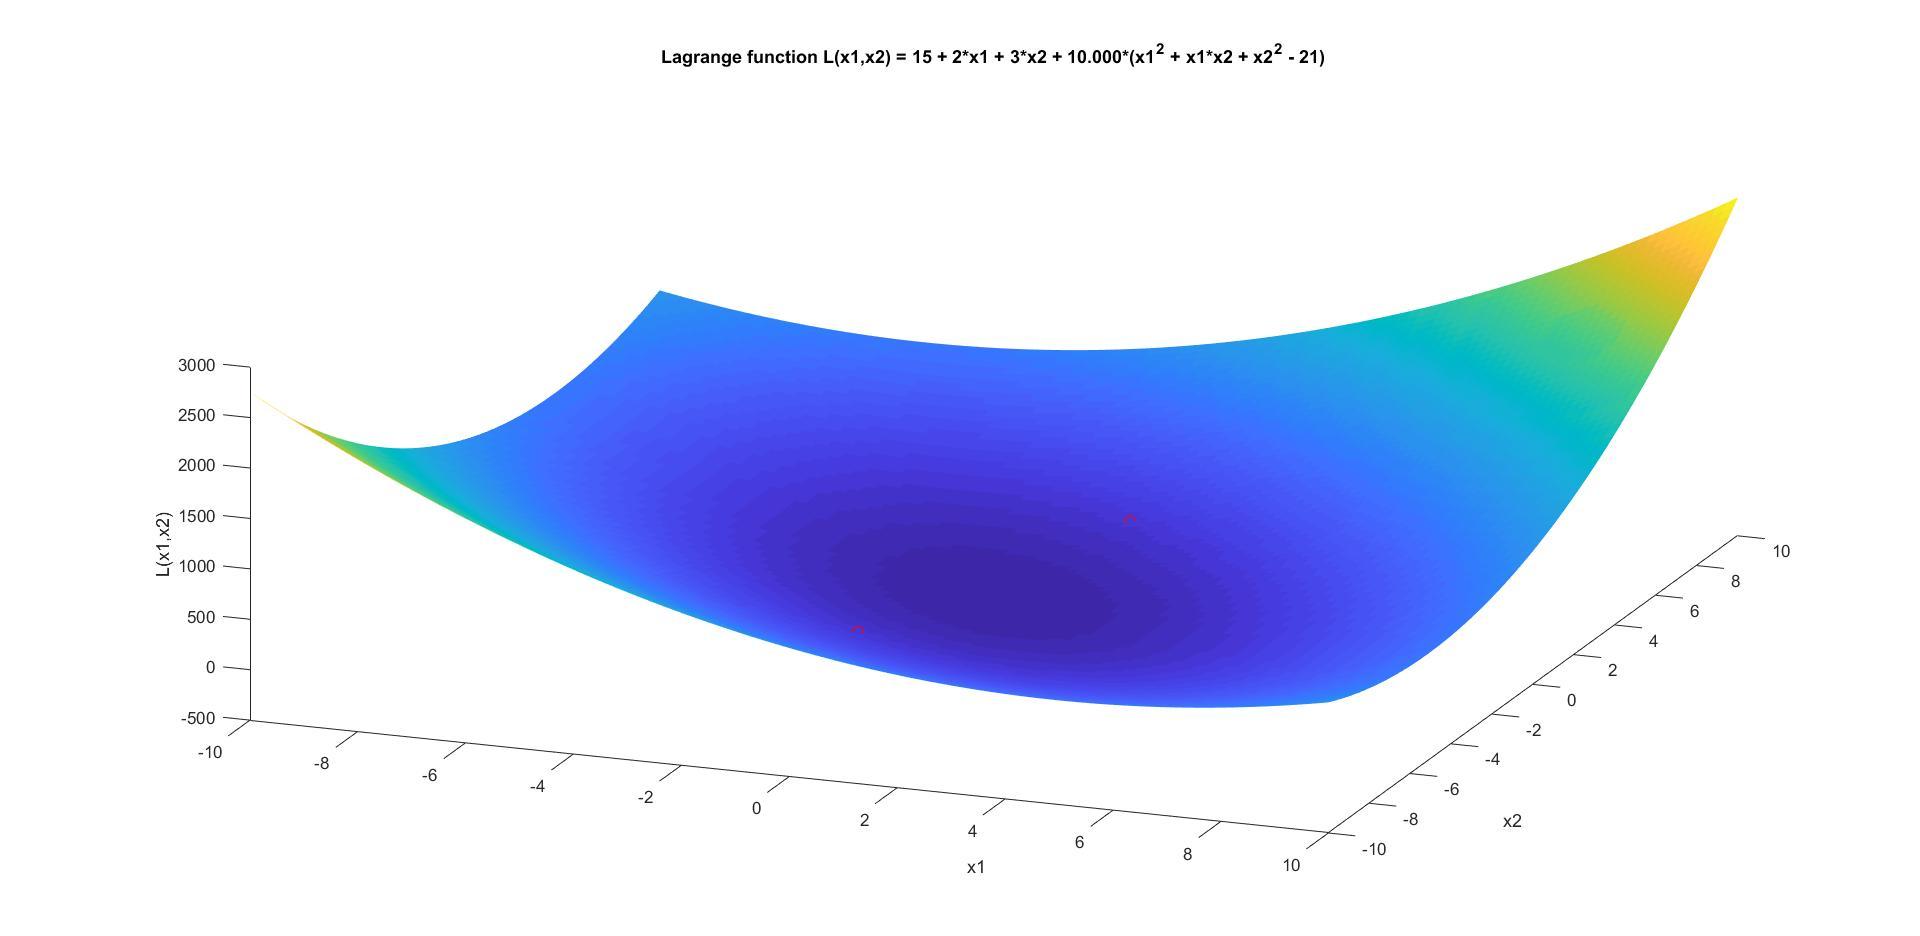
\includegraphics[width=\textwidth]{LagrangeMultiplerMethod/LagrangeMethod_equation_lambda=10.jpg}
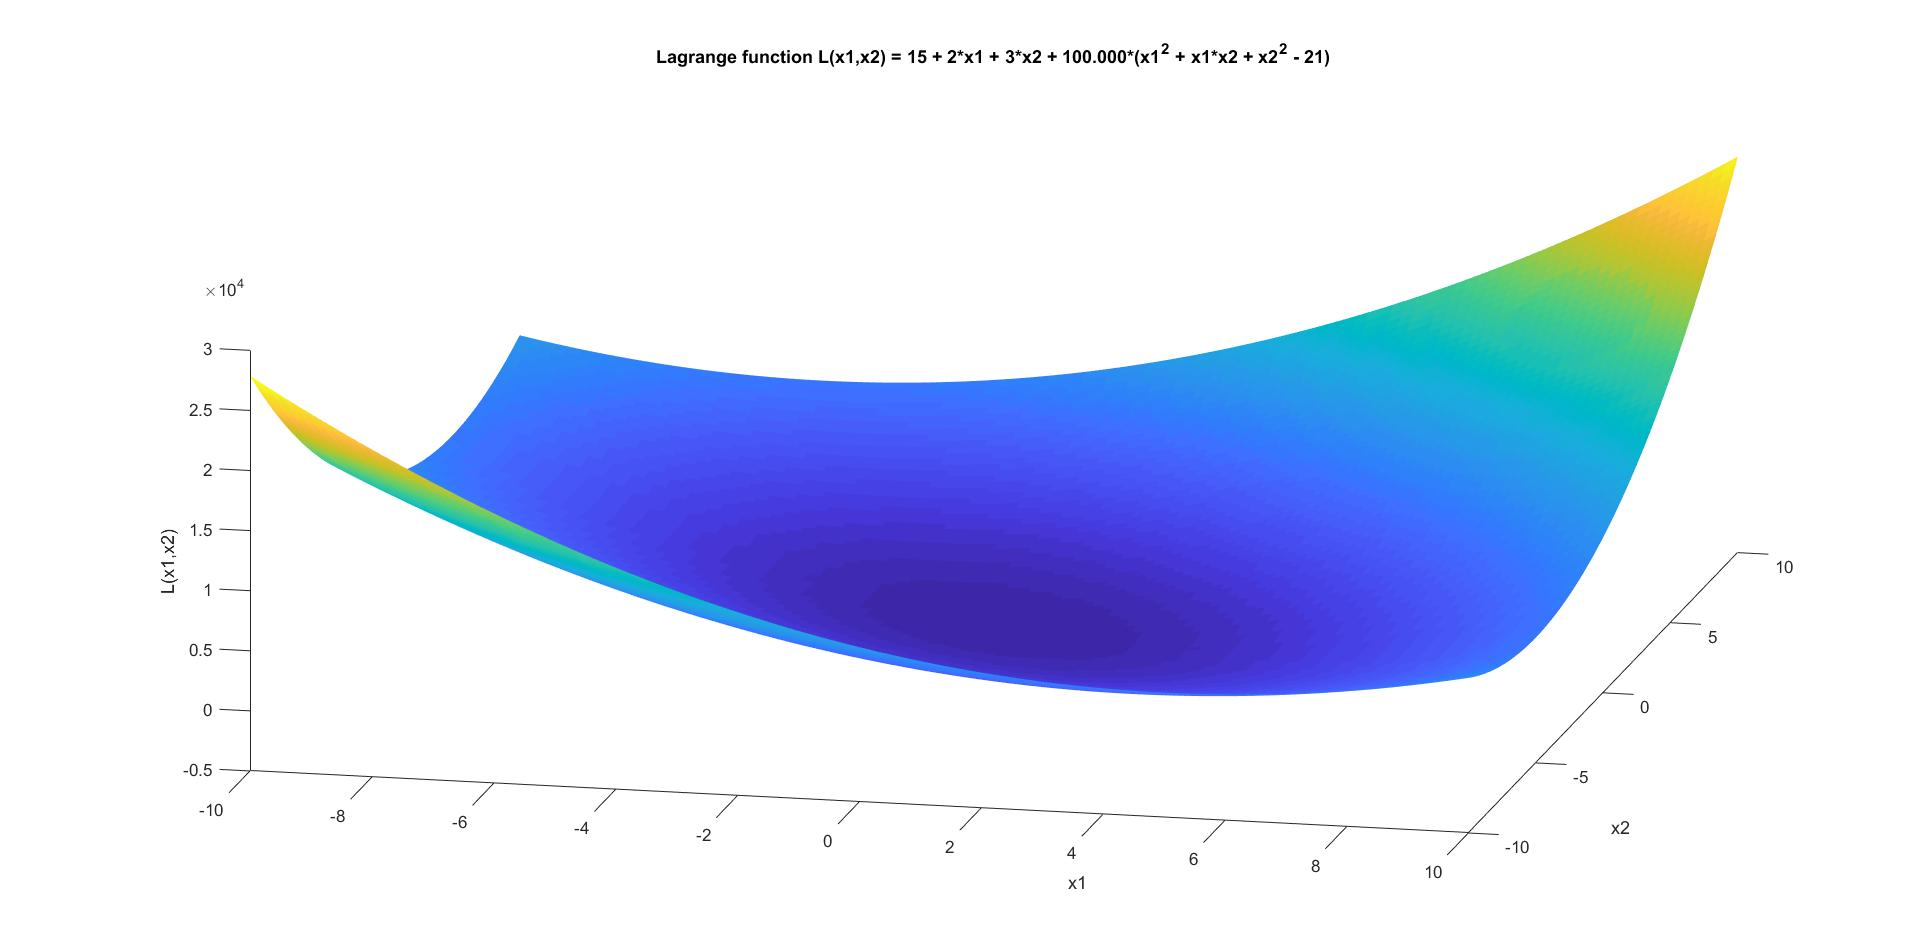
\includegraphics[width=\textwidth]{LagrangeMultiplerMethod/LagrangeMethod_equation_lambda=100.jpg}
\caption{Lagrange multiplier function $L(x_1,x_2,\lambda) = f(x_1,x2) + \lambda*h(x_1,x_2)$ for sequence of $\lambda$ values $[10,100]$).}
\end{figure}

It may be seen that with change of multiplier $\mu$ value superposition of objective function $f(\vec{x})$ and constraints function $h(\vec{x})$ are switching in phase, so position of global minimum (dark blue color) is changing place too. 

\subsection{Gradient of Lagrange Multipler function}

Comparing gradient of Lagrange Multipler unconstrained function to zero, step depends on solving to get points for which objective function value is optima

\begin{equation}\left \{
\begin{tabular}{lcl}
$\frac{\partial{L}}{\partial{x_1}} = 0$ & $\Leftrightarrow$ & $2+\lambda*(2x_1+x_2)=0$\\
$\frac{\partial{L}}{\partial{x_2}} = 0$ & $\Leftrightarrow$ & $3+\lambda*(x_1 + 2x_2)=0$\\
$\frac{\partial{L}}{\partial{\lambda}} = 0$ & $\Leftrightarrow$ & $h(x_1,x_2)=0$\\
\end{tabular}\right
\end{equation}

Notice that in last partial derivative over $\lambda$ term is reduced to initial equality constraint $h(\vec{x})$.

From this one obtains

\begin{equation}\left \{
\begin{tabular}{l}
$\lambda = \frac{-2}{2*x_1 + x_2};$\\
$\lambda = \frac{-3}{x_1 + 2*x_2};$\\
\end{tabular}\right
\label{eq:gradLagrange}
\end{equation}

Here function variables are in denominators, so it is necessary to check if optima do not happens in points corresponding to this terms. First performed is checking for denominator 1 : $2*x_1 + x_2 = 0$ then separately for denominator 2 : $x_1 + 2*x_2 = 0$.

\subsubsection{Check for variables in denominator 1}

If $2x_1 + x_2 = 0$ then $x_2 = -2x_1$. Inserting this to constraint function and comparing to zero (according to third partial derivative) $h(x_1,x_2=-2x_1) = x_1^2 + x_1*(-2x_1) + (-2x_1)^2 - 21 = 0$, after algebraic modifications $x_1^2 -2x_1^2 + 4x_1^2 - 21 = 0$, $2x_1^2=21$ one obtains roots of as:

\begin{equation}\left \{
\begin{tabular}{l}
$x_1 = \pm\sqrt{7};$\\
$x_2 = \mp2\sqrt{7};$\\
\end{tabular}\right
\end{equation}

which gives two points:
\begin{itemize}
    \item $(\sqrt{7},-2\sqrt{7})$ with function value $f(\sqrt{7},-2\sqrt{7})=15-4\sqrt{7}\approx 4.41$;
    \item $(-\sqrt{7},2\sqrt{7})$ with function value $f(-\sqrt{7},2\sqrt{7})=15+4\sqrt{7}\approx26$.
\end{itemize} 

\subsubsection{Check for variables in denominator 2}

If $x_1 + 2x_2 = 0$ then $x_1 = -2x_2$. Inserting this to constraint function and comparing to zero (according to third partial derivative) $h(x_1=-2x_2,x_2=) = (-2x_2)^2 + x_2*(-2x_2) + x_2^2 - 21 = 0$, after algebraic modifications $4x_2^2 -2x_2^2 + x_2^2 - 21 = 0$, $3x_2^2=21$ one obtains roots of as:

\begin{equation}\left \{
\begin{tabular}{l}
$x_1 = \mp2\sqrt{7};$\\
$x_2 = \pm\sqrt{7};$\\
\end{tabular}\right
\end{equation}

which gives two points:
\begin{itemize}
    \item $(-2\sqrt{7},\sqrt{7})$ with function value $f(-2\sqrt{7},\sqrt{7})=15+2(-2\sqrt{7})+3\sqrt{7}=15-\sqrt{7}\approx 12$;
    \item $(2\sqrt{7},-\sqrt{7})$ with function value $f(2\sqrt{7},-\sqrt{7})=15+4\sqrt{7}-3\sqrt{7}=14+\sqrt{7}\approx18$.
\end{itemize} 

\subsubsection{Continuation of solving gradient of Lagrange function for roots}

From this points \ref{eq:gradLagrange} comparing terms by $\lambda$ values $\frac{-3}{x_1 + 2*x_2} = \frac{-2}{2*x_1 + x_2}$, then simplifying to $6x_1+3x_2 = 2x_1+4_x_2$ and switching sides obtained is relation between variables $x_2 = 4x_1$. Substituting variables in equality constraint $h(x_1,4x_1) = x_1^2 + 4x_1^2+16x_1^2-21=0$ then reducing $21x_1^2=21$ from which $x_1^2=1$ and finally

\begin{equation}\left \{
\begin{tabular}{l}
$x_1 = \pm1;$\\
$x_2 = \pm4;$\\
\end{tabular}\right
\end{equation}

which gives two points:
\begin{itemize}
    \item $(1,4)$ with function value $f(1,4) = 15 + 2 + 3*4 = 29$
    \item $(-1,-4)$ with function value $f(-1,-4) = 15 - 2 - 12 = 1$
\end{itemize}

\subsection{Results of Lagrange Multipler formula}

Obtained points and their functions values may be grouped in table below (first point is maxima, second is minima). Both points are reaching conditions given by equality constraints, what one may check by $h(1,4)=0$ and $h(-1,-4)=0$. 

\begin{table}[h]
\centering
\begin{tabular}{l | c | c | c }
\lambda & x_1 & x_2 & $f_p(\vec{x};\mu)$\\
\hline \hline
    -1/3&	1.000&	4.000&	29\\
    1/3&	-1.000&	-4.000& 1\\
\end{tabular}
\caption{OUTPUT : Optima points and function $f(\vec{x},\lambda)$ values obtained with Lagrange Method for $\lambda=1/3$}
\label{tab:lagrangeOutput}
\end{table}

\begin{figure}[H]
\label{fig:lagrangeEquationFigs}
\centering
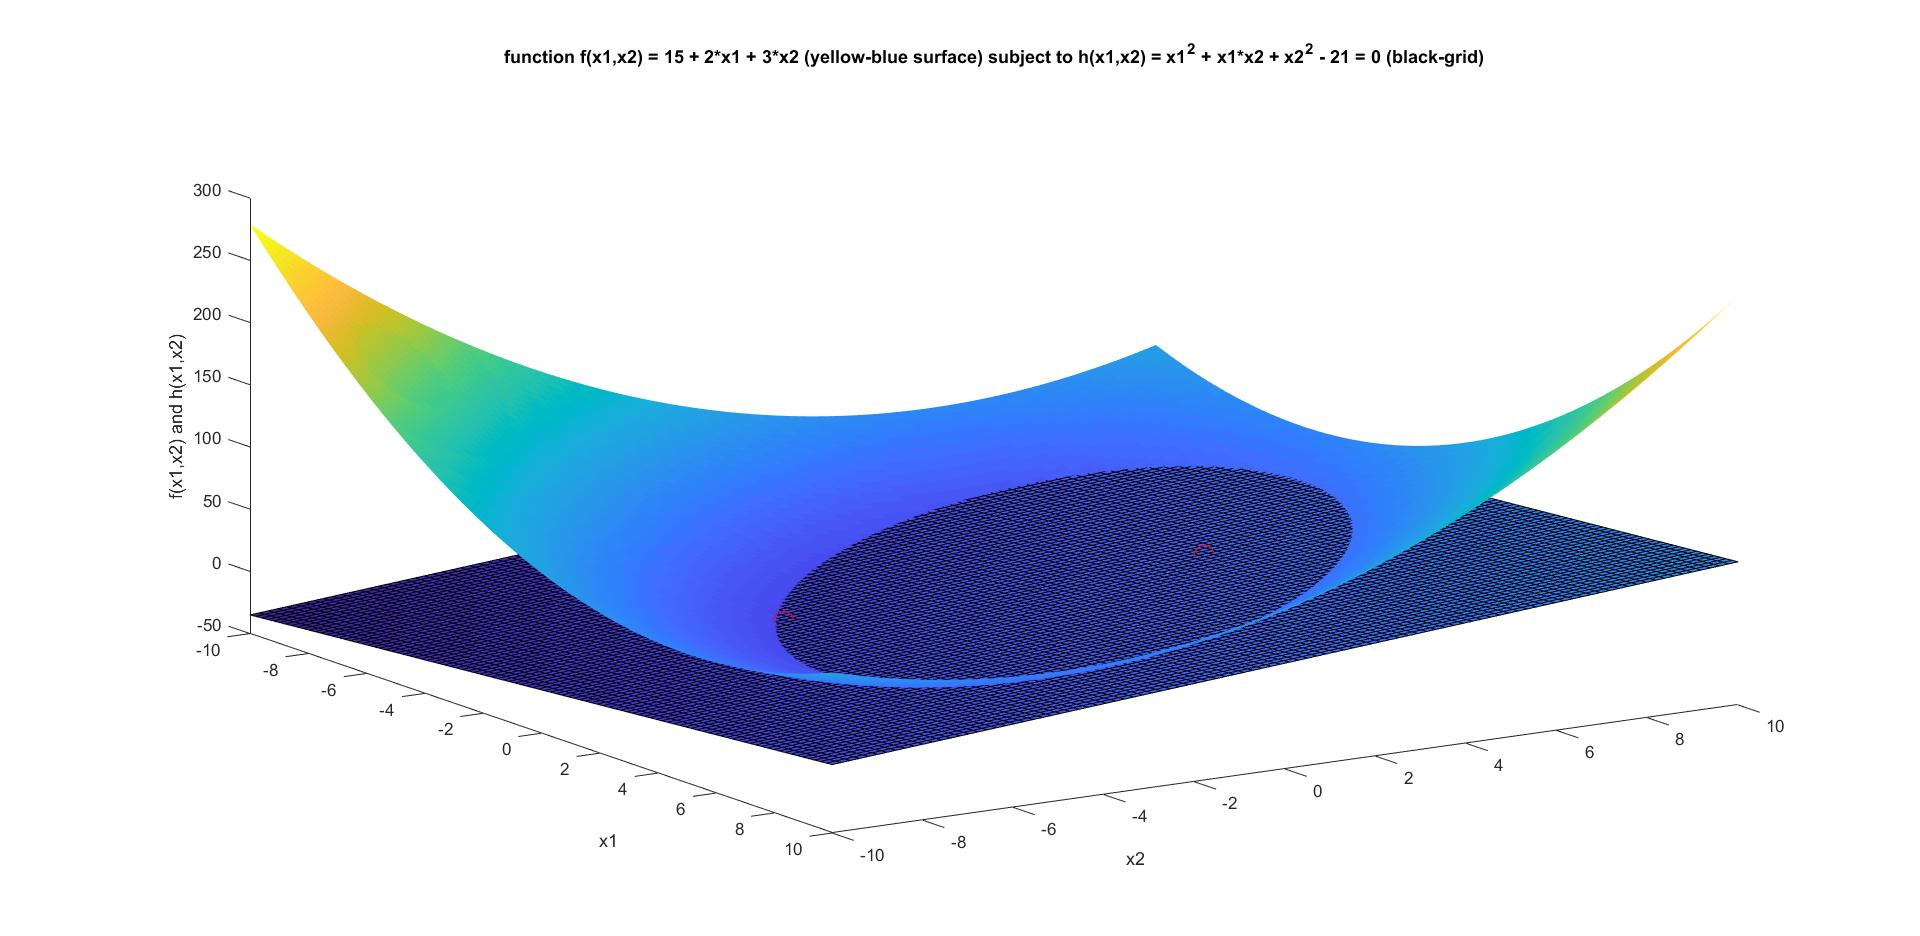
\includegraphics[width=\textwidth]{LagrangeMultiplerMethod/LagrangeMethod_solved.jpg}
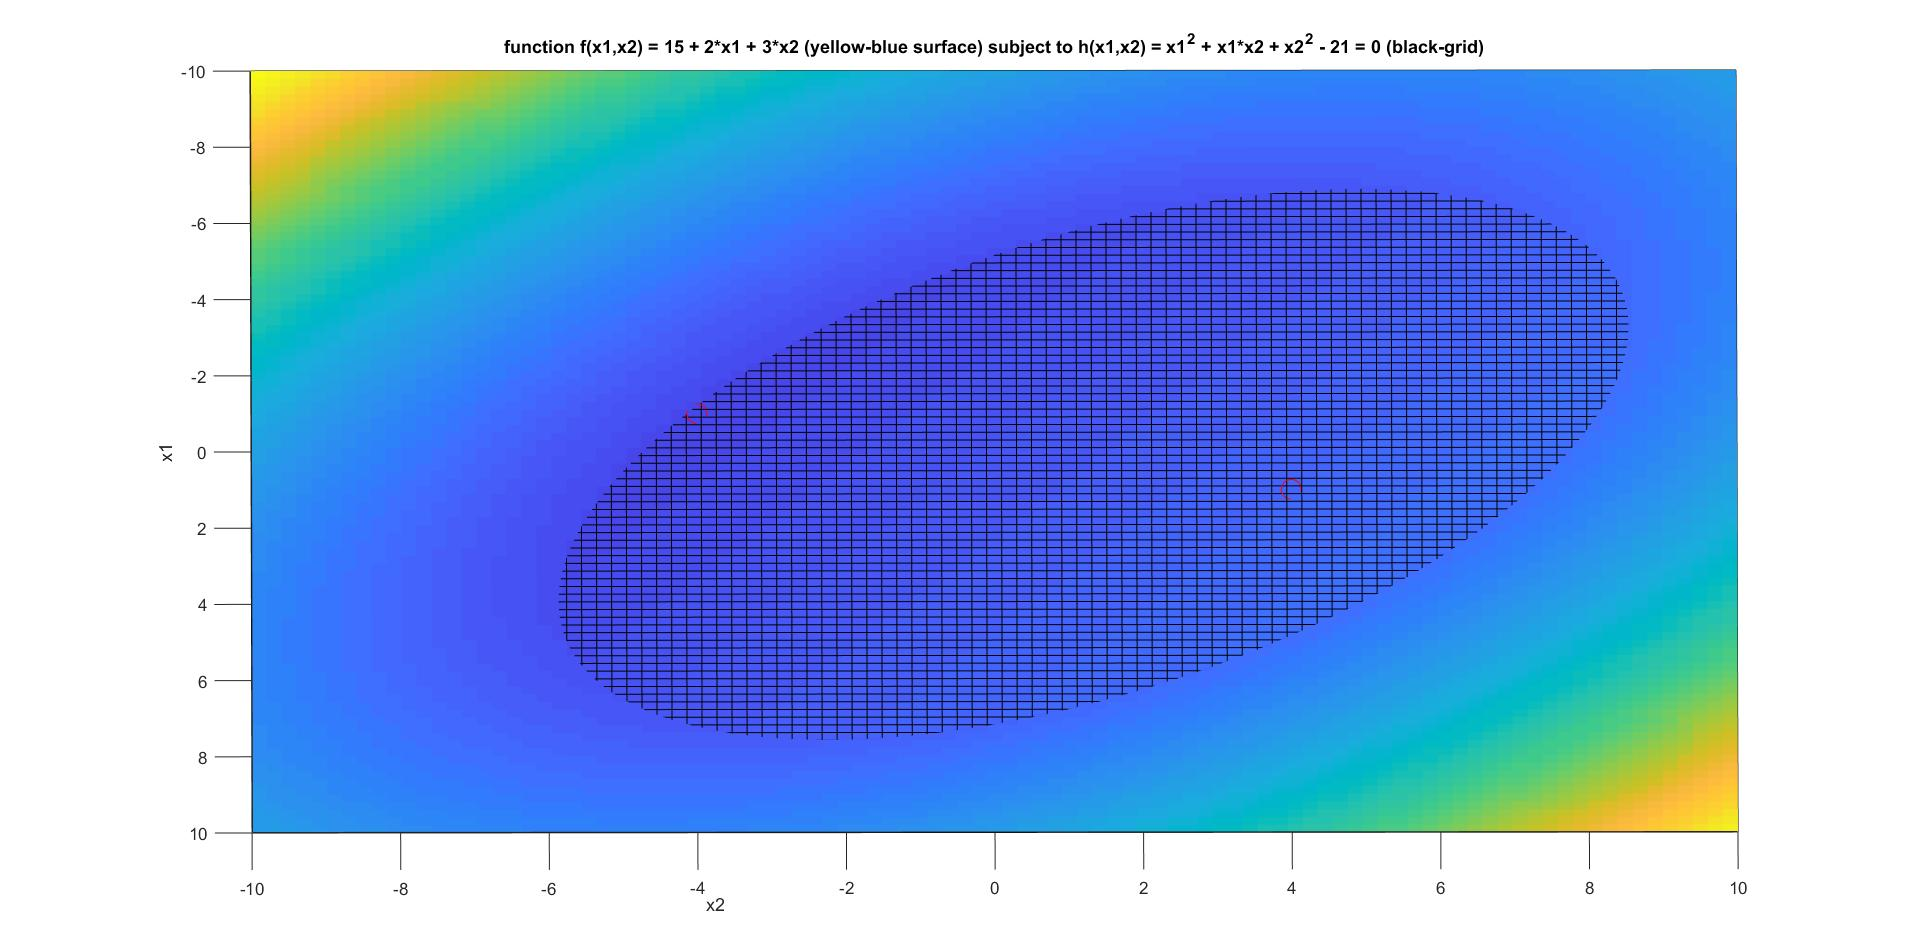
\includegraphics[width=\textwidth]{LagrangeMultiplerMethod/LagrangeMethod_solved_view(0,90).jpg}
\caption{Optima points and function $f(\vec{x},\lambda)$ values obtained with Lagrange Method for $\lambda=1/3$, where point (1,4) with value $f(x_1,f_2)=29$ is maxima and point (-1,-4) with value $f(x_1,f_2)=1$ is minima.}
\end{figure}


\end{document}

